% -*- Mode:TeX -*-

%% The documentclass options along with the pagestyle can be used to generate
%% a technical report, a draft copy, or a regular thesis.  You may need to
%% re-specify the pagestyle after you \include  cover.tex.  For more
%% information, see the first few lines of mitthesis.cls. 

%\documentclass[12pt,vi,twoside]{mitthesis}
%%
%%  If you want your thesis copyright to you instead of MIT, use the
%%  ``vi'' option, as above.
%%
%\documentclass[12pt,twoside,leftblank]{mitthesis}
%%
%% If you want blank pages before new chapters to be labelled ``This
%% Page Intentionally Left Blank'', use the ``leftblank'' option, as
%% above. 

%\documentclass[12pt]{mitthesis}
%\documentclass[12pt,singlespace,twoside]{mitthesis}
\documentclass[12pt,twoside]{mitthesis}
%\documentclass[12pt,oneside]{mitthesis}
%\usepackage{lgrind}
%**********************************************************************
%* Niets toevoegen aan dit bestand zonder toestemming van uw promotor *
%**********************************************************************
\documentclass[12pt,a4paper,oneside]{book}

%%%%%%%%%%%%%%%%%%%%%%%%%%%%%%%%%%%%%%%%%%%%%%%%%%%%%%%%%%%%%%%%%%%%%%%%%%%%%%%%%%
%% Volgende regel activeren voor eReader output:
%\usepackage[papersize={130mm,180mm},margin=2mm]{geometry}

%% Volgende regel activeren voor A4 output (bovenstaande terug afzetten)
\usepackage{a4wide} % Iets meer tekst op een bladzijde
%%%%%%%%%%%%%%%%%%%%%%%%%%%%%%%%%%%%%%%%%%%%%%%%%%%%%%%%%%%%%%%%%%%%%%%%%%%%%%%%%%

%% Packages %%
\usepackage{a4wide}                     % Iets meer tekst op een bladzijde
\usepackage[dutch]{babel}               % Voor nederlandstalige woordsplitsing (en chapter hoofdingen)
\usepackage{amsmath}                    % Uitgebreide wiskundige mogelijkheden
\usepackage{url}                        % Om urls te verwerken
\usepackage{graphicx}                   % Om figuren te kunnen verwerken
\usepackage[latin1]{inputenc}           % Om niet ascii karakters te kunnen typen
\usepackage[pagebackref=true]{hyperref}
\usepackage{listings}                   % improve the code environments
%\usepackage{lmodern}
%\usepackage[T1]{fontenc}
\usepackage{textcomp}
\usepackage{pdfpages}                   % Om pdf documenten in te kunnen voegen (titelpagina)
\usepackage{lipsum}                     % Om lorem ipsum in te voegen
\usepackage{sty/eukdate}                % Om de datum in te voegen 
\usepackage[DoggensLenny]{sty/fncychap} % Added for nicer formatting: (kaders rond titels)
\usepackage{fix-cm}
\usepackage{parskip}                    % Geen inspringing aan het begin van een alinea
%\usepackage{sectsty}
\usepackage{mdwlist}
\usepackage{sty/eukdate}                % Om data in te voegen
\usepackage{caption}
\usepackage{float}                      % Om afbeelding geforceerd op een plek te plaatsten met 'H' parameter
\restylefloat{figure}
\usepackage{multirow}                   % Weergave van complexere tabellen
\usepackage[scaled]{sty/inconsolata}    % Instelling lettertype
\usepackage{verbatim}

\hypersetup{                            % Markup for links in text, final versie enkel met zwarte links!!  %%
    colorlinks = false,                 %false=rode kaders rond tekst, true=links in de tekst zelf in kleur
    linkcolor = black,
    anchorcolor = black,
    citecolor = blue,
    filecolor = black,
    urlcolor = black
}

\renewcommand*\familydefault{\sfdefault}                        % Only if the base font of the document is to be sans serif
%\allsectionsfont{\usefont{OT1}{phv}{bc}{n}\selectfont}
  
\hyphenpenalty=5000                                             % Minder snel woorden splitsen
  \tolerance=1000

%% Custom commands %%
\newcommand{\npar}{\par \vspace{2.3ex plus 0.3ex minus 0.3ex}}  % Enkele mm vertikale ruimte openlaten
\newcommand{\ntpar}{\par \vspace{1.3ex plus 0.3ex minus 0.3ex}}
\newcommand{\nhpar}{\par \vspace{4.3ex plus 0.3ex minus 0.3ex}}

\newcommand{\HRule}{\rule{\linewidth}{0.5mm}}                   % Horizontale lijn

\setcounter{tocdepth}{2}                                        % weergeven tot subsection in table of contents

% \usepackage[final]{sty/TODO}           %TODO package (build error als er nog een todo in het document staat)
%\usepackage[silent]{sty/TODO}           %TODO package (geen output, om een tussentijdse draft zonder de 'todos' te maken)
\usepackage{sty/TODO}                    %TODO package (standaard modus)


\usepackage{eso-pic}
\newcommand\BackgroundPic{%
\put(0,0){%
\parbox[b][\paperheight]{\paperwidth}{%
\vfill
\centering
% 
\includegraphics[width=\paperwidth,height=\paperheight]{figures/titelpagina_ap_lowestres.jpg}
% 
\includegraphics[width=\paperwidth,height=\paperheight]{figures/titelpagina_ap_lowres.jpg}

\includegraphics[width=\paperwidth,height=\paperheight]{figures/titelpagina_ap_mediumres.jpg}

\vfill
}}\hfill
}

\newcommand\BackgroundPicAP{%
\put(220,-372){%
\parbox[b][\paperheight]{\paperwidth}{%
\vfill
\centering

\includegraphics[width=0.44\paperwidth,height=0.075\paperheight,keepaspectratio]{figures/AP.png}
\vfill
}}
\hfill
}

%*************************************************************************************
%* Plaats eventuele extra toegevoegde packages hier (na toestemming van uw promotor) *
%*************************************************************************************




\pagestyle{plain}

%% This bit allows you to either specify only the files which you wish to
%% process, or `all' to process all files which you \include.
%% Krishna Sethuraman (1990).

%\typein [\files]{Enter file names to process, (chap1,chap2 ...), or `all' to process all files:}
%\def\all{all}
%\ifx\files\all \typeout{Including all files.} \else \typeout{Including only \files.} \includeonly{\files} \fi

\begin{document}
%\fontencoding{LY1}\fontfamily{ACaslonPro}\mdweight

\tongjisetup{
  %******************************
  % 注意:
  %   1. 配置里面不要出现空行
  %   2. 不需要的配置信息可以删除
  %******************************
  %
  %=====
  % 秘级
  %=====
  secretlevel={保密},
  secretyear={2},
  %
  %=========
  % 中文信息
  %=========
  % 题目过长可以换行(推荐手动加入换行符,这样就可以控制换行的地方啦)。
  ctitle={同济大学学位论文 \LaTeX{} 模板\\使用示例说明与参考},
  cheadingtitle={同济大学学位论文 \LaTeX{} 模板使用示例说明与参考},    %用于页眉的标题,不要换行
  cauthor={同济人},  
  studentnumber={201804},
  cmajorfirst={工学},
  cmajorsecond={电子控制计算机},
  cdepartment={同济大学Linux用户组},
  csupervisor={陈杰 教授}, 
  % 如果没有副指导老师或者校外指导老师,把{}中内容留空即可,或者直接注释掉。
  cassosupervisor={裴刚 教授~(校外)}, % 副指导老师
  % 日期自动使用当前时间,若需手动指定,按如下方式修改:
  % cdate={\zhdigits{2018}年\zhnumber{11}月},
  % 没有基金的话就注释掉吧。
  cfunds={(本论文由我要努力想办法撑到两行的著名国家杰出青年基金 (No.123456789) 支持)},
  %
  %=========
  % 英文信息
  %=========
  etitle={A Simple Sample of Tongji Thesis\\ Using \tongjithesis{}}, 
  eauthor={Tongji Ren},
  emajorfirst={Gong Xue},
  emajorsecond={DianziControlComputerScience},
  edepartment={TONGJILUG},
  % 日期自动使用当前时间,若需手动指定,按如下方式修改:
  % edate={November,\ 2018},
  efunds={(Supported by the Natural Science Foundation of China for\\ Distinguished Young Scholars, Grant No.123456789)},    
  esupervisor={Prof. Jie Chen},
  eassosupervisor={Prof. Gang Pei (XiaoWai)}
  }

% 定义中英文摘要和关键字
\begin{cabstract}  
  论文的摘要是对论文研究内容和成果的高度概括。摘要应对论文所研究的问题及其研究目
  的进行描述,对研究方法和过程进行简单介绍,对研究成果和所得结论进行概括。摘要应
  具有独立性和自明性,其内容应包含与论文全文同等量的主要信息。使读者即使不阅读全
  文,通过摘要就能了解论文的总体内容和主要成果。

  论文摘要的书写应力求精确、简明。切忌写成对论文书写内容进行提要的形式,尤其要避
  免“第 1 章……;第 2 章……;……”这种或类似的陈述方式。

  本文介绍同济大学论文模板 \tongjithesis{} 的使用方法。本模板符合学校的硕士、
  博士论文格式要求。

  本文的创新点主要有:
  \begin{itemize}
    \item 用例子来解释模板的使用方法;
    \item 用废话来填充无关紧要的部分;
    \item 一边学习摸索一边编写新代码。
  \end{itemize}

  关键词是为了文献标引工作、用以表示全文主要内容信息的单词或术语。关键词不超过 5
  个,每个关键词中间用分号分隔。(模板作者注:关键词分隔符不用考虑,模板会自动处
  理。英文关键词同理。)
\end{cabstract}

\ckeywords{\TeX, \LaTeX, CJK, 模板, 论文}

\begin{eabstract}
   An abstract of a dissertation is a summary and extraction of research work
   and contributions. Included in an abstract should be description of research
   topic and research objective, brief introduction to methodology and research
   process, and summarization of conclusion and contributions of the
   research. An abstract should be characterized by independence and clarity and
   carry identical information with the dissertation. It should be such that the
   general idea and major contributions of the dissertation are conveyed without
   reading the dissertation.

   An abstract should be concise and to the point. It is a misunderstanding to
   make an abstract an outline of the dissertation and words ``the first
   chapter'', ``the second chapter'' and the like should be avoided in the
   abstract.

   Key words are terms used in a dissertation for indexing, reflecting core
   information of the dissertation. An abstract may contain a maximum of 5 key
   words, with semi-colons used in between to separate one another.
\end{eabstract}

\ekeywords{\TeX, \LaTeX, CJK, template, thesis}
\pagestyle{plain}
  % -*- Mode:TeX -*-
%% This file simply contains the commands that actually generate the table of
%% contents and lists of figures and tables.  You can omit any or all of
%% these files by simply taking out the appropriate command.  For more
%% information on these files, see appendix C.3.3 of the LaTeX manual. 
\tableofcontents
\newpage
\listoffigures
\newpage
\listoftables



%now start the fancy headings
\pagestyle{fancyplain}
\addtolength{\headheight}{\baselineskip}
%add a nice little line underneath the heading
%\renewcommand{\headrulewidth}{0.6pt}


\chapter{}
\chapter{Related Works}


\chapter{}
\chapter{Implementation}



\clearpage
\appendix
%\addcontentsline{toc}{part}{Appendix}

\chapter{Abbreviations and reference data}

\section{Basic molecular biology data}

\begin{itemize}
\item     Figure~\vref{fig:aas} shows structures and abbreviations for the
    20 naturally occurring amino acids.  The abbreviations shown in
    the figure are used consistently throughout this thesis.

\item     Figure~\vref{fig:bases} shows structures and abbreviations for the
    four nucleotides found in DNA and RNA, and urysil, which is
    found only in RNA

    \item     Table~\vref{table:codonTable} shows the standard codon table
    that translates from three letter nucleotide sequences to the
    corresponding amino acid during the process of mRNA translation.
\end{itemize}


        \begin{figure}[ptbh]
        \centering
        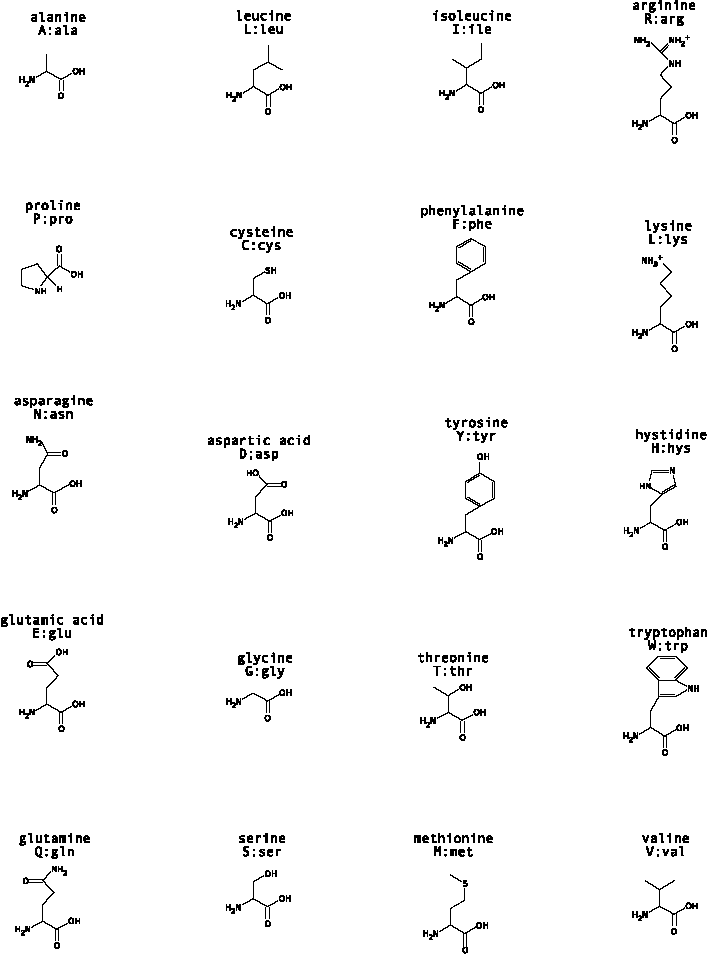
\includegraphics[width=\textwidth]{Body/Images-appa/aas.pdf}
        \caption[Amino acid structures and abbreviations]{Amino acid structures and abbreviations.  The figure shows the chemical
structure of the 20 naturally occurring amino acids and their three letter and
one letter abbreviations.}
        \label{fig:aas} \end{figure}


.
        \begin{figure}[bthp]
        \centering
        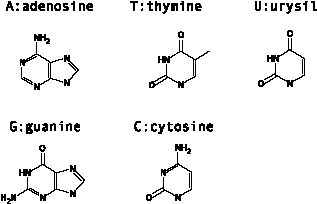
\includegraphics{Body/Images-appa/bases.pdf}
        \caption[Nucleotide base structures and abbreviations]{Nulceotide base structures and abbreviations.}
        \label{fig:bases} \end{figure}



    \begin{table}[tbph]
    \caption[Standard codon table]{Standard codon table.  The table
    should be interpreted by reading the first and second
    nucleotides off of the vertical axis on the left, and reading
    the final nucleotide off of the horizontal axis at the top.
    For example, the amino acid corresponding to the three
    nucleotide sequence \texttt{AAG} is \texttt{Arg}, or arginine.
    }\label{table:codonTable}
    \centering
\begin{verbatim}
                  A      C      G      U
             _____________________________
        AA  |    Lys    Asn    Lys    Asn
   F    AC  |    Thr    Thr    Thr    Thr
   i    AG  |    Arg    Ser    Arg    Ser
   r    AU  |    Ile    Ile    MET    Ile
   s P  CA  |    Gln    His    Gln    His
   t o  CC  |    Pro    Pro    Pro    Pro
     s  CG  |    Arg    Arg    Arg    Arg
   & i  CU  |    Leu    Leu    Leu    Leu
     t  GA  |    Glu    Asp    Glu    Asp
   S i  GC  |    Ala    Ala    Ala    Ala
   e o  GG  |    Gly    Gly    Gly    Gly
   c n  GU  |    Val    Val    Val    Val
   o    UA  |     .     Tyr     .     Tyr
   n    UC  |    Ser    Ser    Ser    Ser
   d    UG  |     .     Cys    Trp    Cys
        UU  |    Leu
\end{verbatim}

    \end{table}


\clearpage

\section{Supplementary data and analyses}

\subsection{Position weight matrix computation and matching}\label{section:pwmCode}

The code shown below is a simple Python script used to compute a
position weight matrix.  The script can be copied from this text and
run on most personal computers.  After the code, I present a brief
example of how this should be run, using the yeast 3' splice sites
shown in Figure~\vref{fig:yeast}.

\begin{singlespace}
\small
\verbatiminput{Body/Images-appa/searchPwm.py}
\normalsize
\end{singlespace}

\begin{singlespace}
\small
\verbatiminput{Body/Images-appa/pwm-run.txt}
\normalsize
\end{singlespace}

\subsection{Antimicrobial design data}

    Figure~\vref{fig:synth1ms} shows the gas and mass spectra for a
    peptide designed in Chapter~\ref{chapter:amps}.  See
    Section~\vref{section:preliminary}.

        \begin{figure}[htbp]
        \centering
        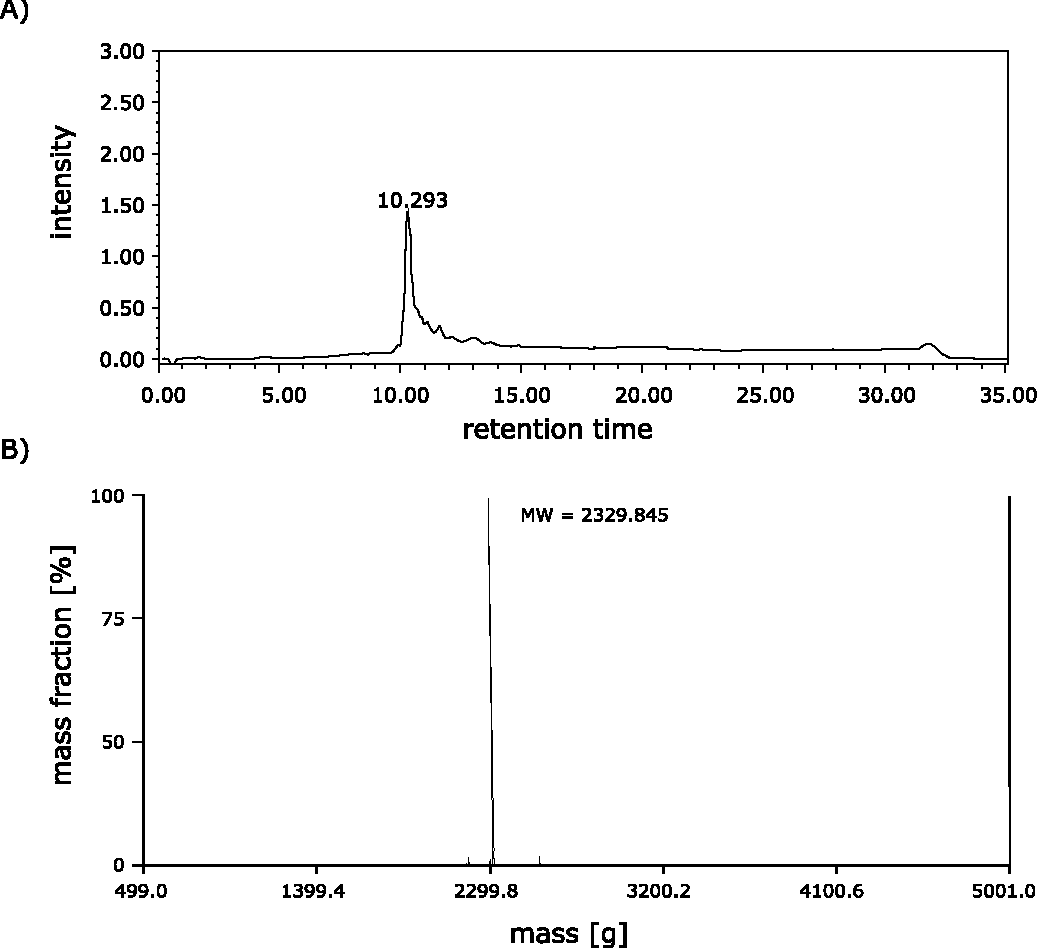
\includegraphics[width=\textwidth]{Body/Images-appa/synth1-spectra.pdf}
        \caption[Gas and mass spectra for the synth--1 peptide]{
        Gas and mass spectra for the synth--1 peptide.  As the
        figure shows, the peptide appears well above  the 85\% purity
        threshold.  This peptide was designed using our preliminary,
        sensitive approach for designing antimicrobial peptides.
        However, the peptide was shown to have undetectable activity
        under good experimental conditions, prompting the more
        focused, specific approach for designing AmPs.
        }
        \label{fig:synth1ms}
        \end{figure}

\import{./Body/appb/}{appb.tex}
%\chapter{Bioinformatics and handwriting/speech recognition: unconventional applications of similarity search tools}
\section{Introduction}
	Bioinformatics has benefited immensely from tools and techniques imported
	from other disciplines.  Markov models used for gene--finding have
	their origin in information science, neural networks are imported
	from machine learning, and the countless clustering methods used
	for analyzing microarray data are from a wide variety of fields.

	Sequence alignment tools are no exception to this trend;
	however, within bioinformatics, they have reached
	new levels of speed and sophistication.  Tools,
	such as Blast~\cite{altschul1990basic,altschul1997gapped}
	and FastA~\cite{pearson1998improved}, are used routinely to search
	through a database for sequences (DNA or protein) that are
	similar to a query sequence.  Over the years, these tools have
	been optimized for speed by employing a number of heuristic
	shortcuts to the dynamic programming algorithms on which
	they are based.  Even searches in very large databases,
	such as Swiss--Prot/TrEMBL~\cite{bairoch2000swiss-prot} or
	GenBank~\cite{benson2000genbank}, take only a few seconds
	for queries of small to moderate size.	This is substantially
	faster than the time required for a rigorous Smith--Waterman
	search~\cite{waterman1984efficient}.  In light of the remarkably
	speed and accuracy that characterize these algorithms, it is 
	intriguing to investigate other applications where similarity
	search tools might be of material importance.  In this work, we present two
	alternative applications of these fast sequence alignment tools
	outside the domain of bioinformatics: handwriting recognition and
	speech recognition.

	The dynamic handwriting recognition problem is to recognize
	handwriting from a touch tablet as found on personal
	digital assistants (PDAs), for example Palm Pilots, or tablet
	PCs~\cite{tappert1990thestate}.  These writing tablets sample
	the position of a pen as a function of time to produce a series of
	($x,y$) points that are used by handwriting recognition algorithms to
	determine which character was written.	An excellent review of the
	most common algorithms is available from Plamodon and Srihari, 2000.
	These include feature analysis, curve matching, Markov models, and
	elastic matching, the last of which is based on dynamic programming
	and is related to both Blast and FastA.

	To apply similarity search concepts to the handwriting recognition
	problem, we represented the path of a PDA pen as a protein
	sequence by translating the ($x,y$) points into a string of
	amino acids.  Using the protein representation of handwriting
	samples, we were able to classify unknown samples with FastA. 
	This is analogous to the problem of protein annotation using
	similarity searching: given a protein (a written character)
	of unknown function, we annotated the protein by searching for
	similar sequences (characters with similar ($x,y$) paths).

	We applied the same sequence alignment approach to speech
	recognition.  Automated phone services, security checkpoints,
	and computer dictation software employ some form of speech
	recognition.  Common speech recognition methods include feature
	recognition, neural networks, hidden Markov models, dynamic
	programming~\cite{ney2000progress} and a variety of other statistical
	and signal processing algorithms.  A good review of these techniques
	and more is available from Juang \& Furui, 2000.  For this problem,
	we represented digital speech recordings as sequences of amino
	acids, and used a database of annotated recordings to classify
	unknown recordings.

	In the following section, we describe the data sets used for the
	handwriting recognition and speech recognition problems.  Then,
	we detail how these data were represented using strings of amino
	acids and how we used FastA to annotate unknown samples in four
	handwriting and speech recognition experiments.  We compare our
	results to more traditional methods of handwriting and speech
	recognition and, finally, we discuss ways of improving upon the
	results and extending sequence alignment to other classification
	problems.

		\begin{figure}[t!]
				\centering
				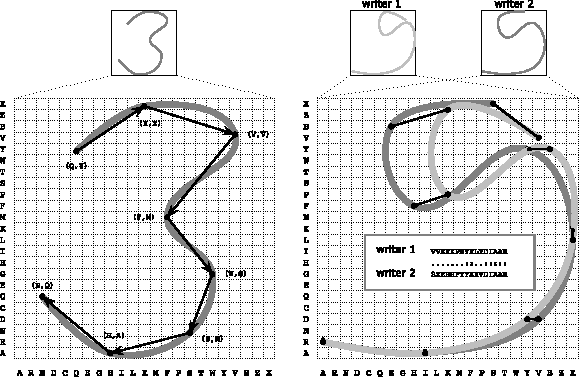
\includegraphics[width=\textwidth]{Body/Images-appc/digits.pdf}
			\caption{Projection of a digit written with
					a PDA stylus into protein space.
					Concatenating the set of
					points gives a protein sequence
					representative of the digit.
					In this case, the sequence is
					\texttt{QYKXVVFMWGSNHANQ}.%
					An alignment of nines from two
					different writers.  The boxes at
					the top show the input from each
					writer and the large grid show the
					superposition of the two handwritten
					digits.  The FastA alignment between
					the protein representations of the
					two digits is shown in the center.
				Two visualizations of the handwriting
				recognition problem.  In both cases the
				$x$ and $y$ axes are divided into 23 parts
				corresponding to the columns and rows in
				an amino acid scoring matrix.  The eight
				sampled points from the digit are cast from
				$x,y$ space into protein space by assigning
				amino acid coordinates to each point.
			}\label{fig:pda}\label{fig:pdaAlign}
		\end{figure}

		\begin{table*}[t!] 
			\centering
			\caption[fooba]{Results for the handwriting and
				speech recognition problems described
				in the text.  For each experiment,
				the misclassification is the percent of
				sequences in the unknown set for which the
				digit or letter was not predicted correctly.}
			\subtable[
				Handwriting recognition results.
			]{
\begin{tabular}{ccc}\hline\hline
Experiment & Classification & \parbox{4.8cm}{\centering \vspace{1mm}Classification in\\
Alimoglu \& Alpaydin, 1996\vspace{1mm}}  \\ \hline
1 & 97.34\%  & 97.80\% \\
2 & 99.64\% & n/a \\
%3 & 0.46\% & n/a \\
\hline\hline
\end{tabular}
} \subtable[Speech
				recognition results.
				The second column shows the
				misclassification using the clustering of
				all /ee/ sounding letters as described in the
				text.  ]{ 
\begin{tabular}{cccc}\hline\hline
Experiment & Classification & \parbox{2.5cm}{\vspace{1mm}Classification\\ with clustering\vspace{1mm}} & \parbox{4.5cm}{\centering \vspace{1mm}Classification in\\
Dietterich \& Bakiri, 1995\vspace{1mm}} \\ \hline
1 & 93.84\% & 98.91\%  & 96.73\% \\
2 & 92.61\% & 98.61\% &  n/a \\
%3 & 5.11\% & 0.71\% & n/a \\
\hline\hline
\end{tabular}
 }
			\label{table:results2}\label{table:results1}
		\end{table*}


		\begin{table*}[!b]
		\centering
		\caption[Handwriting Alignment Scoring Matrix]{The scoring matrix used for the handwriting
			and speech recognition FastA alignments.
			Each entry of the scoring matrix, $s_{ij}$, is given by $s_{ij}= 10-(|i-j|)$.
			That is, matching amino acids are given 10 ``points'', amino acids
			that are one off are given 9 points, and so on.  This matrix was used
			in place of the default scoring matrix,  Blosum50~\cite{henikoff1992aminoacid},  for FastA.
			The scoring matrix was found heuristically.  Also, a few experiments indicated that the
			alignments are relatively insensitive to permutations about the form of $s_{ij}$ given above.

		} \label{table:matrix}
		
\tiny
 \begin{tabular}{c@{\hspace{2mm}}c@{\hspace{2mm}}c@{\hspace{2mm}}c@{\hspace{2mm}}c@{\hspace{2mm}}c@{\hspace{2mm}}c@{\hspace{2mm}}c@{\hspace{2mm}}c@{\hspace{2mm}}c@{\hspace{2mm}}c@{\hspace{2mm}}c@{\hspace{2mm}}c@{\hspace{2mm}}c@{\hspace{2mm}}c@{\hspace{2mm}}c@{\hspace{2mm}}c@{\hspace{2mm}}c@{\hspace{2mm}}c@{\hspace{2mm}}c@{\hspace{2mm}}c@{\hspace{2mm}}c@{\hspace{2mm}}c@{\hspace{2mm}}c@{\hspace{2mm}}c}\hline\hline
 & A & R & N & D & C & Q & E & G & H & I & L & K & M & F & P & S & T & W & Y & V & B & Z & X\\ 
A & 10 & 9 & 8 & 7 & 6 & 5 & 4 & 3 & 2 & 1 & 0 & -1 & -2 & -3 & -4 & -5 & -6 & -7 & -8 & -9 & -10 & -11 & -12\\ 
R & 9 & 10 & 9 & 8 & 7 & 6 & 5 & 4 & 3 & 2 & 1 & 0 & -1 & -2 & -3 & -4 & -5 & -6 & -7 & -8 & -9 & -10 & -11\\ 
N & 8 & 9 & 10 & 9 & 8 & 7 & 6 & 5 & 4 & 3 & 2 & 1 & 0 & -1 & -2 & -3 & -4 & -5 & -6 & -7 & -8 & -9 & -10\\ 
D & 7 & 8 & 9 & 10 & 9 & 8 & 7 & 6 & 5 & 4 & 3 & 2 & 1 & 0 & -1 & -2 & -3 & -4 & -5 & -6 & -7 & -8 & -9\\ 
C & 6 & 7 & 8 & 9 & 10 & 9 & 8 & 7 & 6 & 5 & 4 & 3 & 2 & 1 & 0 & -1 & -2 & -3 & -4 & -5 & -6 & -7 & -8\\ 
Q & 5 & 6 & 7 & 8 & 9 & 10 & 9 & 8 & 7 & 6 & 5 & 4 & 3 & 2 & 1 & 0 & -1 & -2 & -3 & -4 & -5 & -6 & -7\\ 
E & 4 & 5 & 6 & 7 & 8 & 9 & 10 & 9 & 8 & 7 & 6 & 5 & 4 & 3 & 2 & 1 & 0 & -1 & -2 & -3 & -4 & -5 & -6\\ 
G & 3 & 4 & 5 & 6 & 7 & 8 & 9 & 10 & 9 & 8 & 7 & 6 & 5 & 4 & 3 & 2 & 1 & 0 & -1 & -2 & -3 & -4 & -5\\ 
H & 2 & 3 & 4 & 5 & 6 & 7 & 8 & 9 & 10 & 9 & 8 & 7 & 6 & 5 & 4 & 3 & 2 & 1 & 0 & -1 & -2 & -3 & -4\\ 
I & 1 & 2 & 3 & 4 & 5 & 6 & 7 & 8 & 9 & 10 & 9 & 8 & 7 & 6 & 5 & 4 & 3 & 2 & 1 & 0 & -1 & -2 & -3\\ 
L & 0 & 1 & 2 & 3 & 4 & 5 & 6 & 7 & 8 & 9 & 10 & 9 & 8 & 7 & 6 & 5 & 4 & 3 & 2 & 1 & 0 & -1 & -2\\ 
K & -1 & 0 & 1 & 2 & 3 & 4 & 5 & 6 & 7 & 8 & 9 & 10 & 9 & 8 & 7 & 6 & 5 & 4 & 3 & 2 & 1 & 0 & -1\\ 
M & -2 & -1 & 0 & 1 & 2 & 3 & 4 & 5 & 6 & 7 & 8 & 9 & 10 & 9 & 8 & 7 & 6 & 5 & 4 & 3 & 2 & 1 & 0\\ 
F & -3 & -2 & -1 & 0 & 1 & 2 & 3 & 4 & 5 & 6 & 7 & 8 & 9 & 10 & 9 & 8 & 7 & 6 & 5 & 4 & 3 & 2 & 1\\ 
P & -4 & -3 & -2 & -1 & 0 & 1 & 2 & 3 & 4 & 5 & 6 & 7 & 8 & 9 & 10 & 9 & 8 & 7 & 6 & 5 & 4 & 3 & 2\\ 
S & -5 & -4 & -3 & -2 & -1 & 0 & 1 & 2 & 3 & 4 & 5 & 6 & 7 & 8 & 9 & 10 & 9 & 8 & 7 & 6 & 5 & 4 & 3\\ 
T & -6 & -5 & -4 & -3 & -2 & -1 & 0 & 1 & 2 & 3 & 4 & 5 & 6 & 7 & 8 & 9 & 10 & 9 & 8 & 7 & 6 & 5 & 4\\ 
W & -7 & -6 & -5 & -4 & -3 & -2 & -1 & 0 & 1 & 2 & 3 & 4 & 5 & 6 & 7 & 8 & 9 & 10 & 9 & 8 & 7 & 6 & 5\\ 
Y & -8 & -7 & -6 & -5 & -4 & -3 & -2 & -1 & 0 & 1 & 2 & 3 & 4 & 5 & 6 & 7 & 8 & 9 & 10 & 9 & 8 & 7 & 6\\ 
V & -9 & -8 & -7 & -6 & -5 & -4 & -3 & -2 & -1 & 0 & 1 & 2 & 3 & 4 & 5 & 6 & 7 & 8 & 9 & 10 & 9 & 8 & 7\\ 
B & -10 & -9 & -8 & -7 & -6 & -5 & -4 & -3 & -2 & -1 & 0 & 1 & 2 & 3 & 4 & 5 & 6 & 7 & 8 & 9 & 10 & 9 & 8\\ 
Z & -11 & -10 & -9 & -8 & -7 & -6 & -5 & -4 & -3 & -2 & -1 & 0 & 1 & 2 & 3 & 4 & 5 & 6 & 7 & 8 & 9 & 10 & 9\\ 
X & -12 & -11 & -10 & -9 & -8 & -7 & -6 & -5 & -4 & -3 & -2 & -1 & 0 & 1 & 2 & 3 & 4 & 5 & 6 & 7 & 8 & 9 & 10\\ \\
\hline\hline\end{tabular}

		\end{table*}

		\begin{figure}[ptbh]
		\centering
		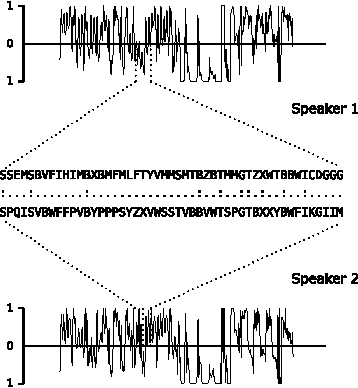
\includegraphics[width=\textwidth]{Body/Images-appc/voice.pdf}
		
			%\scalebox{0.80}{
			%	\footnotesize
			%	\psset{xunit=1cm,yunit=1cm}
\readdata{\dataA}{Figures/voiceSeq1-xy.dat}
\readdata{\dataB}{Figures/voiceSeq2-xy.dat}
\begin{pspicture}(0,0)(10,10)%\showgrid
	\rput(2,9){
		\rput(-1,0){
			\psaxes[tickstyle=bottom, dy=\psyunit,Dy=1,Oy=0,Ox=0,Dx=100](0,0)(0,-1)(8,1)
		}
		\dataplot[plotstyle=line,linecolor=black,linewidth=0.1mm]{\dataA}
	}
	\rput(2,1){
		\rput(-1,0){
			\psaxes[tickstyle=bottom, dy=\psyunit,Dy=1,Oy=0,Ox=0,Dx=100](0,0)(0,-1)(8,1)
		}
		\dataplot[plotstyle=line,linecolor=black,linewidth=0.1mm]{\dataB}
	}
	\rput[l](0.4, 5.5){\normalsize \texttt{SSEMSBVFIHIMBXBMFMLFTYVMMSMTBZBTMMGTZXWTBBWICDGGG}}
	\rput[l](0.4, 5){\normalsize \texttt{:...:.......:...............:..:..::.:..:..:.....}}
	\rput[l](0.4, 4.5){\normalsize \texttt{SPQISVBWFFPVBYPPPSYZXVWSSTVBBVWTSPGTBXXYBWFIKGIIM}}
	\rput(0, 0){
		\psline[linestyle=dotted](4,2)(0.55,4.3)
		\psline[linestyle=dotted](4.4,2)(10.6,4.3)
		\psline[linestyle=dotted](4.4,2)(4.4,1)
		\psline[linestyle=dotted](4.2,2)(4.2,1)
	}
	\rput(0, 0){
		\psline[linestyle=dotted](4,8)(0.55,5.7)
		\psline[linestyle=dotted](4.4,8)(10.6,5.7)
		\psline[linestyle=dotted](4,8)(4,9)
		\psline[linestyle=dotted](4.4,8)(4.4,9)
	}
	\rput[bl](8.5, 8){Speaker 1}
	\rput[tl](8.5, 2){Speaker 2}

		
		
%	\rput(0.8,150){
%		\rotatebox{90}{ \# sequences}
%	}
%	\rput(8.5,150){
%		\rotatebox{-90}{ \# patterns}
%	}
%	\rput(5,0){
%		bootstrapping iterations
%	}


%	number LSWBBTTTTYZXBW SSEMSBVFIHIMBXBMFMLFTYVMMSMTBZBTMMGTZXWTBBWICD
%	       .............. :...:.......:...............:..:..::.:..:..:..
%	number TZXYSMFPYVVVTS SPQISVBWFFPVBYPPPSYZXVWSSTVBBVWTSPGTBXXYBWFIKG
%	250       260       270       280       290       300

%	310       320       330       340       350       360
%	number GGGCIWYFMELKKFTKPLILAAAAAAAAAADWZIHWIDDCCDNRAAAAAAAAAAAAAAAA
%	       ....................:::::::::...... ........::::::::::::::::
%	number IIMKPFIILHGDMSYTIEHEAAAAAAAAARITBTDEMGQEHCRAAAAAAAAAAAAAAAAA

\end{pspicture}

			%	\normalsize
			%}
		\caption[A Voice alignment]{
			An alignment of the spoken--letter ``X'' recorded from two different speakers.
			The plots at the top and bottom are recordings for first and second
			speakers, respectively.  The breakout in the center shows a section of the protein
			projection of each recording and the alignment generated using FastA
			as described in the text.  This example was taken from the first speech
			recognition experiment.  In this case, the bottom recording was the top
			scoring alignment against the top recording.
		}
		\label{fig:voiceAlign}
		\end{figure}

		\begin{figure}[ptbh]
		\centering
		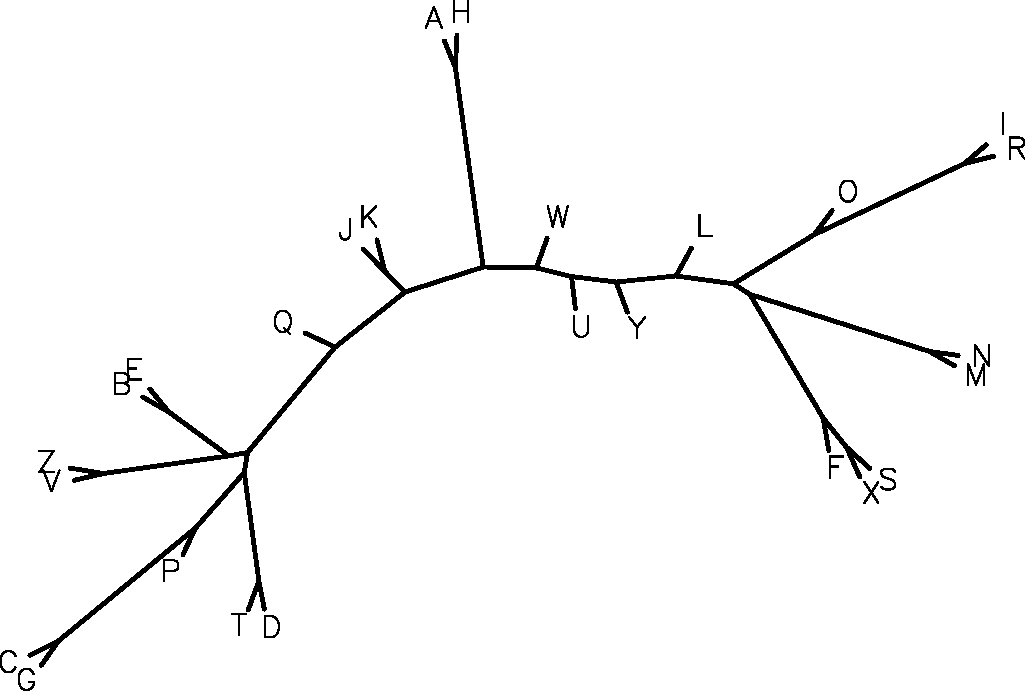
\includegraphics[width=\textwidth]{Body/Images-appc/tree.pdf}
		\caption[A PDA digit]{
			A phylogenetic tree of voice--proteins.
			This tree was created using the
			Phylip~\cite{felsenstein1989phylip} tree drawing
			program from a multiple sequence alignment of
			all 26 voice--proteins from a single speaker.
			The multiple sequence alignment was made using the
			ClustalW~\cite{higgins1992improved} alignment tool,
			with the scoring matrix in Table~\vref{table:matrix}.
			In the tree, similar sounding (homologous) letters
			are grouped near each other.  For example, all the
			letters containing the /ee/ sound [\emph{B, C, D,
			E, G, P, T, V, Z}] are clustered on the left side
			of the tree.
		} \label{fig:tree} \end{figure}



\section{System and Methods}
	\subsection{Handwriting Recognition}
		For our handwriting recognition experiments, we used
		data from Alimoglu and Alpaydin, 1996, available in the
		University of California Irvine repository of machine
		learning databases~\cite{uci1998ucirepository}.  These data
		comprised of 10992 handwritten digits between \emph{0}
		and \emph{9}, written by 44 writers with each writer
		submitting 250 digits (8 samples were discarded by the
		original authors).

		Each digit was written with a stylus pen on a touch tablet,
		which recorded the $x$ and $y$ coordinates of the pen as a
		function of time.  These data were re-sampled such that each
		written digit was represented by a series of eight $(x,y)$
		points, spaced out by a constant arc length over the path of
		the digit.  Then, for each digit, the set of $(x,y)$ points
		were scaled such that the largest axis, usually the $y$ axis,
		ranged from 0 to 1.  By dividing the number line $[0,1]$
		into 23 ``bins'' we translated each of these coordinates
		into a pair of amino acids as shown in Figure~\vref{fig:pda}.
		We concatenated these amino acid pairs to obtain a protein
		sequence representation of each digit: a ``digit--protein.''



		
	\subsection{Speech Recognition}
		For our speech recognition experiments, we used data from
		Deitterich and Bakiri, 1995, %~\cite{dietterich1995solving}
		available in the University of California Irvine repository
		of machine learning databases~\cite{uci1998ucirepository}.
		This data set consisted of 7797 recordings of individuals
		speaking one of the letters \emph{A--Z}.  A total of 150
		speakers each said every letter \emph{A--Z} twice (three
		recordings were discarded by the original authors).
		Then, each recording was processed into a set of 617
		real--valued attributes in the range $[-1,1]$.	A more
		detailed description of the database is available from
		Dietterich \& Bakiri, 1995.%~\cite{dietterich1995solving}.

		By dividing the number line $[-1,1]$ into 23 bins we translated these real numbers into a series
		of amino acids.  For example, the series ``-1.0,-0.55, 0.11, 0.65'' was translated
		to ``{\texttt{AQKY}}''.  We concatenated these amino acids to make a protein representation
		of each recording: a ``voice--protein''.


\section{Results}
	\subsection{Handwriting Recognition}

		We conducted two handwriting recognition experiments.
		In both experiments part of the digit--protein database was assumed to contain a
		``known'' set of digits that was subsequently used to annotate,
		or classify, the remaining ``unknown'' digits.	For our
		first experiment, we used for the known database containing the
		writing of 30 persons (7494 digits) and an unknown database
		with the writing of the remaining 14 persons (3498 digits).
		Using FastA, we searched each sequence from the unknown
		set in the known set and used the top scoring hits to
		annotate the unknown digits.  Searches were carried out
		using the scoring matrix shown in Table~\vref{table:matrix}
		with FastA version 3.4t11 using the default gap open and
		extension penalties, and the following options: \texttt{-p
		-Q -d0 -f-8 -g-1 -H -E1000 -b1}.  An example alignment of
		two handwritten nines from different writers is shown in
		Figure~\vref{fig:pdaAlign}.


		For our second experiment, we used 25\% (2748 digits) of our
		digit--protein database, selected randomly, as the unknown
		set and the remaining 75\% (8244 digits) as our known set.
		Alignments and annotations using FastA were performed as
		in the first experiment.

		The results of the two handwriting recognition
		experiments are shown in Table~\vref{table:results1}.
		In experiment 1, our results are about the same as
		the best k--means clustering results of Alimoglu and
		Alpaydin~\cite{alimoglu1996methods,alimoglu1997combining}.
		This experiment simulates the user--independent
		handwriting recognition problem: the handwriting of one
		group of writers was used to classify digits from a different group.
		In the user--dependent problem, experiment 2, the database
		of known handwritten digits contains samples from all the writers,
		on average.  Thus, for every unknown handwriting sample,
		there is often a close match in the database of known
		samples.  As such, the results of experiment 2 are
		significantly better than those of experiment 1 as shown
		in Table~\vref{table:results1}.



		%In contrast to k--means clustering and other common machine learning techniques for handwriting
		%recognition, there was no explicit training or learning phase of our experiments.  As such, 
		%we included experiment 3, which is a realistic approximation of the recognition problem 
		%on a tablet PC with multiple users.  The results for this experiment are considerably better than
		%experiment 2 because there are relatively more known sequences which can be used for annotating
		%the unknown sequence.

		In experiment 1, the average time for each alignment was
		0.117 seconds per unknown sequence on a 1 gHz Pentium III
		processor.  This is much shorter than the time required to
		write the digits.  Thus sequence alignment could be used
		as a ``real--time'' method for handwriting recognition.
		This high speed, together with the high accuracy for
		user--dependent recognition makes sequence alignment good
		candidate for use on a Tablet PCs, or even PDAs.

	\subsection{Speech Recognition}


		Using the voice--protein database, we conducted two
		experiments, analogous to the two handwriting recognition
		experiments described previously.  First, we used a known
		set consisting of 6238 recordings from 120 speakers and
		an unknown set with 1559 recordings from the remaining 30
		speakers.  Second, we used 25\% (1949 recordings) of the
		voice--protein database, selected randomly, as the unknown
		set and the remaining 75\% (5848 recordings) as the known
		set.  Each of the speech recognition alignments was performed
		using the same scoring matrix and FastA parameters as the
		handwriting recognition experiments.  An example alignment
		of two voice--proteins is shown in Figure~\vref{fig:voiceAlign}.


		The results of the two speech recognition experiments are shown in
		Table~\vref{table:results2}.
		Experiment 1 is compared
		to the best Error Correcting Output Code (ECOC) results of Deitterich
		and Bakiri,
		%~\cite{dietterich1995solving}
		but
		there was no comparison available for experiment 2.	
		The misclassification for experiment 1 was 6.16\%, 
		higher than the ECOC result of 3.27\%.  However, we observed that
		most of the errors were due to rhyming letters, and in particular
		all of the /ee/ sounding characters [\emph{B, C, D, E, G, P, T, V, Z}].
		This indicated that these characters were similar on a sequence level,
		so we constructed a phylogenetic tree of the sequences to study their
		relationship.

	

		A phylogenetic tree of 26 voice--proteins from a single
		speaker is shown in Figure~\vref{fig:tree}.  As the figure
		shows, the protein projections of phonetically similar
		letters tend to be homologous.	Furthermore, letters such
		as \emph{A} and \emph{H}, which have the /ay/ sound at the
		beginning, are more closely related to each other than
		they are to \emph{J} and \emph{K}, which have the /ay/
		sound at the end.  Because the /ee/ sounding letters all
		have /ee/ at the end, they are particularly difficult
		to distinguish from each other.  These letters account
		for a disproportionate majority of the errors in our two
		experiments.  By clustering these letters together such that
		they are considered the same for classification purposes,
		the error in experiment 1 was reduced to 1.09\%.  If the
		original error was evenly distributed between the classes,
		the error would have been reduced only to about 5.5\%.
		This suggests that, although string alignment performs
		poorly for /ee/ sounding characters, it performs well for
		all other characters.


\section{Conclusions}
		This work showed that sequence alignment can be a powerful
		classification tool for problems outside the domain
		of bioinformatics.  In both the handwriting and speech
		recognition problems, we projected real--valued data into
		strings of amino acids and used FastA as a classification
		tool, in a manner analogous to protein annotation.  In the
		case of handwriting recognition, we showed that sequence
		alignment is a viable alternative to traditional methods,
		such as k--means clustering, and is fast enough to be used
		as a real--time recognition method.


		There are many ways to improve upon the results we presented here.
		First, we did not have any explicit training phase for either set of experiments.
		However, there are at least two sequence alignment parameters which can
		be trained: the gap open and extension penalties, and the scoring matrix.
		The optimization of these parameters for protein annotation is well documented
		~\cite{henikoff1993performance,altschul1991amino,henikoff1992aminoacid,dayhoff1979amodel,vogt1995assessment,henikoff2000amino}
		and would be similar for alternative sequence alignment applications such
		as handwriting recognition.  Second, intelligent projection of data
		into strings can greatly improve results.  Here, we used bins of equal
		size to partition the real--valued data into amino acids; however, bins
		of unequal size may improve the resolution between closely related sequences
		and improve classification.  Finally, more customizable sequence alignment tools
		would be very useful.  These tools should take an arbitrary alphabet (Blast
		and FastA are restricted to 23 amino acids) and a user--defined scoring
		matrix (FastA allows user--defined matrices, but Blast does not).

		The potential applications of sequence alignment tools
		outside of bioinformatics are boundless.  Tools such as Blast
		and FastA can be used to quickly classify or search through
		any data that can be projected into a string of characters.
		Of course, these methods will work best with data that is
		of a low dimension.  Our experiments with more complex data
		data, such as color images, suggest that how the data are
		projected into a string is very important with large number
		of dimensions.	However, for simple types of data, such
		as customer purchase histories, black and white images, or
		Internet chat transcripts, we have been able to use sequence
		alignment as a quick and effective classification tool.


%% This defines the bibliography file (main.bib) and the bibliography style.
%% If you want to create a bibliography file by hand, change the contents of
%% this file to a `thebibliography' environment.  For more information 
%% see section 4.3 of the LaTeX manual.
%\bibliographystyle{plainnat}
\bibliographystyle{abbrvnat}

\clearpage
%\addcontentsline{toc}{chapter}{Bibliography}
\bibliography{References/research-new}

%\subsection{密钥导出算法}

在 TLS 1.3 中,不再使用 PRF 算法,而是采用更标准的 HKDF 算法来进行密钥的推导。而且在 TLS 1.3 中对密钥进行了更细粒度的优化,每个阶段或者方向的加密都不是使用同一个密钥。TLS 1.3 在 ServerHello 消息之后的数据都是加密的,握手期间服务器给客户端发送的消息用 server\_handshake\_traffic\_secret 通过 HKDF 算法导出的密钥加密的,Client 发送给 Server 的握手消息是用 client\_handshake\_traffic\-\_secret 通过 HKDF 算法导出的密钥加密的。这两个密钥是通过 Handshake Secret 密钥来导出的,而 Handshake Secret 密钥又是由 PreMasterSecret 和 Early Secret 密钥导出,然后通过 Handshake Secret 密钥导出主密钥 Master Secret。

再由主密钥 Master Secret 导出这几个密钥: client\_application\_traffic\_secret:用来导出客户端发送给服务器应用数据的对称加密密钥。server\_application\_traffic\_s\-ecret:用来导出服务器发送给客户端应用数据的对称加密密钥。resumption\_master\_\\secret:用来生成 PSK。最终 server\_handshake\_traffic\_secret、client\_handshake\_traffic\_\\secret、 client\_application\_\-traffic\_secret、server\_application\_traffic\_secret 这 4 个密钥会分别生成 4 套 write\_key 和 write\_IV 用于对称加密。如果用到 early\_data,还需要 client\_e\-arly\_traffic\_secret,它也会生成 1 套 write\_key 和 write\_IV 用于加密和解密 0-RTT 数据。Key Derivation Function (KDF) 是密码学系统中必要的组件。它的目的是把一个 key 拓展成多个从密码学角度来上说是安全的 key。

TLS 1.3 使用的是 HMAC-based Extract-and-Expand Key Derivation Function 即 HKDF 函数,HKDF 根据 extract-then-expand 设计模式,即 KDF 有 2 大模块。第一个阶段是将输入的 key material 进行 "extracts",得到固定长度的 key,然后第二阶段将这个 key "expands" 成多个附加的伪随机的 key,输出的 key 的长度和个数,取决于指定的加密算法。由于 extract 流程不是必须的,所以 expand 流程可以独立的使用。HMAC 的两个参数,第一个是 key,第二个是 data。data 可以由好几个元素组成,一般用 | 来表示

经过密钥协商得出来的密钥材料的随机性可能不够,协商的过程能被攻击者获知,需要使用一种密钥导出函数来从初始密钥材料(PSK 或者 DH 密钥协商计算出来的 key)中获得安全性更强的密钥。HKDF 正是 TLS 1.3 中所使用的这样一个算法,使用协商出来的密钥材料和握手阶段报文的哈希值作为输入,可以输出安全性更强的新密钥。在 TLS 1.2 中使用的密钥导出函数 PRF 实际上只实现了 HKDF 的 expand 部分,并没有经过 extract,而直接假设密钥材料的随机性已经符合要求。因为 TLS 1.3 对密钥材料进行 extract\_then\_expand,所以这也是为什么 TLS 1.3 比 TLS 1.2 在安全性上更上一层楼的原因。TLS 1.3 中的所有密钥都是由 HKDF-Extract(salt, IKM) 和 Derive-Secret(Secret, Label, Messages) 联合导出的。其中 Salt 是当前的 secret 状态,输入密钥材料(IKM)是要添加的新 secret 。在 TLS 1.3 中,两个输入的 IKM 是: PSK 或者 (EC)DHE 共享 的 secret。一旦计算出了从给定 secret 派生出的所有值,就应该删除该 secret。

% TLS 1.3 中的 Finished 并不算是整个握手中的第一条加密消息,作用和 TLS 1.2 是相同的,它对提供握手和计算密钥的身份验证起了至关重要的作用。 Authentication 消息的计算统一采用以下的输入方式: 1. 要使用证书和签名密钥 2. 握手上下文由哈希副本中的一段消息集组成 3. Base key 用于计算 MAC 的密钥。Finished 子消息根据 Transcript-Hash(Handshake Context, Certificate, CertificateVerify) 的值得出的 MAC 。使用从 Base key 派生出来的 MAC key 计算的 MAC 值。用于计算 Finished 消息的密钥是使用 HKDF,Base Key 是 server\_handshake\_traffic\_ secret 和 client\_handshake\_traffic\_secret。

% 如果使用同一个密钥加密大量的数据,攻击者有几率可以通过记录所有密文并找出特征,逆推出对称加密密钥。因此需要引进一个密钥同步更新的机制,该机制同时也使用 HKDF 算法,在旧密钥的基础上衍生出新一轮的密钥。当加密的报文达到一定长度后,双方也需要发送 KeyUpdate 报文重新计算加密密钥。KeyUpdate 握手消息用于表示发送方正在更新其自己的发送加密密钥。任何对等方在发送 Finished 消息后都可以发送此消息。在接收 Finished 消息之前接收 KeyUpdate 消息的,实现方必须使用 "unexpected\_message" alert 消息终止连接。发送 KeyUpdate 消息后,发送方应使用新一代的密钥发送其所有流量。收到 KeyUpdate 后,接收方必须更新其接收密钥。

% 下一代 application\_traffic\_secret 计算方法如下

% \lstinputlisting[language=C,xleftmargin=2em,framexleftmargin=1.5em]{./code/key-update.txt}

% \newpage
\end{document}

